\documentclass{article}
\usepackage{hyperref}
\usepackage{listings}
\usepackage{color}
\usepackage{xcolor}
\usepackage{geometry}
\usepackage{graphicx}
\usepackage{amsmath}
\usepackage{caption}
\usepackage{subcaption}
\usepackage{syntax}
\geometry{margin=1in}
\pdfminorversion=6

\newcommand\TODO[1]{\textcolor{red}{TODO: #1}}

\newcommand\header[2]{
    \begin{center}
        {\large
        UCSD CSE 291 (Differentiable Programming) Assignment #1: \\
        \vspace{0.3cm}
        \Large
        #2}
    \end{center}
}

\definecolor{dkgreen}{rgb}{0,0.6,0}
\definecolor{gray}{rgb}{0.5,0.5,0.5}
\definecolor{mauve}{rgb}{0.58,0,0.82}
\lstset{frame=tb,
        aboveskip=3mm,
        belowskip=3mm,
        showstringspaces=false,
        columns=flexible,
        basicstyle={\small\ttfamily},
        numbers=none,
        numberstyle=\tiny\color{gray},
        keywordstyle=\color{blue},
        commentstyle=\color{dkgreen},
        stringstyle=\color{mauve},
        breaklines=true,
        breakatwhitespace=true,
        tabsize=2
}

\hypersetup{colorlinks=true}


\begin{document}

\header{1}{Forward mode automatic differentiation}

\section{Total derivatives}

In our first homework, we will implement what is known as the ``forward mode'' automatic differentiation in loma for generating code that computes the derivatives.
Specifically, given a (differentiable) function $f: \mathbb{R}^n \rightarrow \mathbb{R}^m$, we will automatically generate its \href{https://en.wikipedia.org/wiki/Total_derivative}{total derivative} $df: \mathbb{R}^n \times \mathbb{R}^n \rightarrow \mathbb{R}^m$. 
The total derivative $df(\mathbf{x}, \mathbf{dx})$ (noticed that it takes two inputs $\mathbf{x}$ and $\mathbf{dx}$ instead of only one!) is defined as the best linear approximation at point $\mathbf{x}$:
\begin{equation}
\lim_{\mathbf{dx} \rightarrow 0} \frac{\left\|f(\mathbf{x} + \mathbf{dx}) - \left(f(\mathbf{x}) + df(\mathbf{x}, \mathbf{dx})\right)\right\|}{\left\|\mathbf{dx}\right\|} = 0,
\label{eq:totalderiv}
\end{equation}
where $df(\mathbf{x}, \mathbf{dx})$ is linear over the $\mathbf{dx}$ argument (but not necessarily linear over the $x$ argument).

We can get the partial or directional derivatives that we are more used to from the total derivative function $df$. For example, we can apply a ``one-hot'' vector $\mathbf{v}_i$ for computing the partial derivative of the $i$-th component of the input:
\begin{equation}
\frac{\partial}{\partial x_i} f(\mathbf{x}) = df(\mathbf{x}, \mathbf{v}_i), v_{i,j} = \begin{cases}
1 & \text{ if } i = j, \\
0 & \text{ otherwise}.
\end{cases}
\end{equation}

For notational convienence, we further define a function $Df: \mathbf{R}^n \times \mathbf{R}^n \rightarrow \mathbb{R}^m \times \mathbb{R}^m$ that combines the outputs of function $f$ and its total derivative $df$:
\begin{equation}
Df(x, dx) = \left(f(x), df(x, dx)\right).
\end{equation}

We will focus on straight-line code for this homework, that is, code without if-else statements, loops, and function calls to other loma functions. We will relax this assumption in Homework 3. 

The key idea of forward-mode automatic differentiation is the \textbf{chain rule}. Let
\begin{equation}
    f(x) = g(h(x)).
\end{equation}
Then,
\begin{equation}
    Df(x, dx) = Dg(Dh(x, dx)).
\end{equation}
(Try proving this using the definition of total derivative!)

Therefore, if we have a straight-line code of a function \lstinline{f}
\begin{lstlisting}[language=Python]
def f(x : In[float], y : In[float]) -> float:
    z0 : float = h(x, y)
    z1 : float = g(z0)
    return z1
\end{lstlisting}
We can automatically synthesize its \lstinline{Df} by 1) replacing all datatypes \lstinline{float} with a new struct \lstinline{_dfloat} that stores both the primal value and the total derivative, and 2) replacing all function calls with their own ``Df'':
\begin{lstlisting}[language=Python]
class _dfloat:
    val : float
    dval : float

def Df(x : In[_dfloat], y : In[_dfloat]) -> _dfloat:
    z0 : _dfloat = Dh(x, y)
    z1 : _dfloat = Dg(z0)
    return z1
\end{lstlisting}
We can recursively perform this transformation to function \lstinline{h} and \lstinline{g}, then we are done!

Now, we need to provide the terminal cases of our recursive transformation. Notice that these \lstinline{h} and \lstinline{g} functions can be \emph{any} function. For example, if $h(x, y) = x + y$, then we can derive (from the definition of total derivative) that $Dh(x, y, dx, dy) = (x + y, dx + dy)$. 

Here, we provide the list of terminal cases of the basic operations in loma:
\begin{equation}
\begin{aligned}
\text{DConstant}(c) &= (c, 0) \\
\text{DVariable}(x, dx) &= (x, dx) \\
\text{DAdd}(x, y, dx, dy) &= (x + y, dx + dy) \\
\text{DSub}(x, y, dx, dy) &= (x - y, dx - dy) \\
\text{DMul}(x, y, dx, dy) &= (x \cdot y, x \cdot dy + y \cdot dx) \\
\text{DDiv}(x, y, dx, dy) &= \left(\frac{x}{y}, \frac{x \cdot dy - y \cdot dx}{y^2}\right) \\
\text{DSin}(x, dx) &= \left(\sin(x), \cos(x) \cdot dx\right) \\
\text{DCos}(x, dx) &= \left(\cos(x), -\sin(x) \cdot dx\right) \\
\text{DSqrt}(x, dx) &= \left(\sqrt{x}, \frac{dx}{2\sqrt{x}}\right) \\
\text{DPow}(x, y, dx, dy) &= \left(x^y, dx \cdot \left(y \cdot x^{y-1}\right) + dy \cdot \left(x^y \log(x)\right)\right) \\
\text{DExp}(x, dx) &= \left(\exp{x}, \exp{x} \cdot dx\right) \\
\text{DLog}(x, dx) &= \left(\log{x}, \frac{dx}{x}\right) \\
\text{Dfloat2int}(x, dx) &= \left(\text{float2int}(x), 0\right)
\end{aligned}
\end{equation}

\section{Forward-mode automatic differentiation in loma}

Our goal is this homework is to transform loma functions to their derivatives. In loma, the total derivative of a function is declared as follows:
\begin{lstlisting}[language=Python]
def f(x : In[float]) -> float:
    # ...

df = fwd_diff(f) # df has type _dfloat -> _dfloat
\end{lstlisting}

Loma should automatically generate the content of \lstinline{df}, so the programmer does not have to implement it themselves.

The transformation will happen in \lstinline{autodiff.py} and \lstinline{forward_diff.py}. \textbf{Your task is to fill in the blanks in the \lstinline{forward_diff} function in \lstinline{forward_diff.py}. Use \lstinline{hw_tests/hw1/test.py} to test your implementation. If you pass all tests, you get full points. Each test is weighted equally.}

\subsection{Transformation of types}
We (well, I) have implemented most of this part for you, but you should still understand this part for your implementation. We define a basic type for differentiation: \lstinline{_dfloat}:
\begin{lstlisting}[language=Python]
class _dfloat:
    val : float
    dval : float
\end{lstlisting}
For convienence, we have also provided a constructor \lstinline{make__dfloat}:
\begin{lstlisting}[language=Python]
def make__dfloat(val : In[float], dval : In[float]) -> _dfloat:
    ret : _dfloat
    ret.val = val
    ret.dval = dval
    return ret
\end{lstlisting}

For integers, the corresponding differential type is still \lstinline{int}.
The \lstinline{_dfloat} type represents the primal values and total derivatives of floats. For a general struct with id \lstinline{X}, we synthesize a new differential struct with id \lstinline{_dX}, where we convert the types of all its members to the differential type. For example, for the following types:
\begin{lstlisting}[language=Python]
class Foo:
    x : int
    y : float
    z : Bar

class Bar:
    a : float
    b : int
\end{lstlisting}
We will generate the following new types to represent the primal values and total derivatives:
\begin{lstlisting}[language=Python]
class _dFoo:
    x : int
    y : _dfloat
    z : _dBar

class _dBar:
    a : _dfloat
    b : int
\end{lstlisting}

For a function definition, we transform all argument types and return type to their \lstinline{_d} counterparts. For example, for the following function \lstinline{f}:
\begin{lstlisting}[language=Python]
def f(x : float, y : Foo) -> Bar:
    # ...

df = fwd_diff(f)
\end{lstlisting}
\lstinline{df} would have the type:
\begin{lstlisting}[language=Python]
def df(x : _dfloat, y : _dFoo) -> _dBar:
    # ...
\end{lstlisting}

Finally, loma introduces a type modifier \lstinline{Diff[]} that allows one to specify the \lstinline{_d} counterpart of a type. For example, \lstinline{Diff[float]} resolves to the type \lstinline{_dfloat}, and \lstinline{Diff[Foo]} resolves to the type \lstinline{_dFoo}. 

We have implemented these transformations except for the function definition part in \lstinline{resolve_diff_types()} in \lstinline{autodiff.py}.

\subsection{Transformation of statements and expressions}
This is the main thing you will need to figure out for this homework. We will use an \lstinline{IRMutator} to visit a \lstinline{FunctionDef} node that represents the primal function, and transform it to the derivative function. You should be able to do this by only modifying the \lstinline{FwdDiffMutator} in \lstinline{forward_diff.py}. I recommend you to try to pass the tests one-by-one and incrementally build up your implementation. Here, we briefly describe each test and what you need to implement to pass the tests.

\paragraph{test_identity} The test asks you to transform an identity function.
\begin{lstlisting}[language=Python]
def identity(x : In[float]) -> float:
    return x

d_identity = fwd_diff(identity)
\end{lstlisting}
\lstinline{d_identity} should be something like:
\begin{lstlisting}[language=Python]
def d_identity(x : In[_dfloat]) -> _dfloat:
    return make__dfloat(x.val, x.dval)
\end{lstlisting}
You will need to implement \lstinline{mutate_function_def}, \lstinline{mutate_var}, and \lstinline{mutate_return} for the transformation. You may find the \lstinline{type_to_diff_type} useful for transforming the function signatures. 

\lstinline{mutate_function_def(self, node)} takes a node that is itself a \lstinline{loma_ir.FunctionDef} (see Homework 0 for the definition), and should return another \lstinline{loma_ir.FunctionDef} that is the forward differentiation transformed version. Read \lstinline{irmutator.py} to see how to create a \lstinline{FunctionDef}. \lstinline{mutate_var(self, node)} instead takes a node that is a \lstinline{loma_ir.Var}. We recommend returning a tuple here: the first element of the tuple being the primal value (\lstinline{x.val} in this case), and the second element being the differential (\lstinline{x.dval} in this case). You might want to use \lstinline{loma_ir.StructAccess} to access the \lstinline{.val} and \lstinline{.dval} members. Finally, \lstinline{mutate_return} takes the return statement and transform it. If you choose to return a tuple from \lstinline{mutate_var}, you will need to assemble them to return the result. We recommend to assemble the results by building a \lstinline{loma_ir.Call} to \lstinline{make__dfloat}, with the primal and differential expressions being the two arguments.

\paragraph{test_constant} This time, you are asked to transform a constant function.
\begin{lstlisting}[language=Python]
def constant(x : In[float]) -> float:
    return 2.0

d_constant = fwd_diff(constant)
\end{lstlisting}
\lstinline{d_constant} should be something like:
\begin{lstlisting}[language=Python]
def d_constant(x : In[_dfloat]) -> _dfloat:
    return make__dfloat(2.0, 0.0)
\end{lstlisting}
You will need to implement \lstinline{mutate_const_float} to pass this test. Like \lstinline{mutate_var}, we recommend to return the primal and differential expressions as a tuple here as well.

\paragraph{test_plus, test_subtract, test_multiply, test_divide} These tests asks you to implement the derivatives of some binary operations:
\begin{lstlisting}[language=Python]
def plus(x : float, y : float) -> float:
    return x + y

d_plus = fwd_diff(plus)

def subtract(x : float, y : float) -> float:
    return x - y

d_subtract = fwd_diff(subtract)

def multiply(x : float, y : float) -> float:
    return x * y

d_multiply = fwd_diff(multiply)

def divide(x : float, y : float) -> float:
    return x / y

d_divide = fwd_diff(divide)
\end{lstlisting}
To pass this test, implement \lstinline{mutate_add}, \lstinline{mutate_sub}, \lstinline{mutate_mul} and \lstinline{mutate_div}.

As a reference, here's what \lstinline{d_plus} should look like:
\begin{lstlisting}[language=Python]
def d_plus(x : _dfloat, y : _dfloat) -> _dfloat:
    return make__dfloat(x.val + y.val, x.dval + y.dval)
\end{lstlisting}

\lstinline{mutate_add(self, node)} takes a \lstinline{loma_ir.BinaryOp} node as input. You can use \lstinline{node.left} and \lstinline{node.right} to access the two children nodes. Like \lstinline{mutate_var} and \lstinline{mutate_const_float}, we recommend returning a tuple of two expressions, one is the primal and one is the differential. \lstinline{mutate_sub}, \lstinline{mutate_mul} and \lstinline{mutate_div} should work similarly.

\paragraph{test_declare} Now we will start to have variable declaration. You'll need to implement \lstinline{mutate_declare} to pass this test.

You are asked to transform this code:
\begin{lstlisting}[language=Python]
def declare(x : In[float], y : In[float]) -> float:
    z0 : float = x + y
    z1 : float = z0 + 5.0
    z2 : float = z1 * z0
    return z2

d_declare = fwd_diff(declare)
\end{lstlisting}

You should turn it into something like:
\begin{lstlisting}[language=Python]
def d_declare(x : In[_dfloat], y : In[_dfloat]) -> _dfloat:
    z0 : _dfloat = make__dfloat(x.val + y.val, x.dval + y.dval)
    z1 : _dfloat = make__dfloat(z0.val + 5.0, z0.dval + 0.0)
    z2 : _dfloat = make__dfloat(z1.val * z0.val, z1.dval * z0.dval + z1.val * z0.dval)
    return make__dfloat(z2.val, z2.dval)
\end{lstlisting}
Each line is turned from a \lstinline{float} declaration into a \lstinline{_dfloat} declaration. The implementation should be similar to \lstinline{return}.

\paragraph{test_assign and test_side_effect} Next, we test variable assignment. You'll need to implement \lstinline{mutate_assign} to pass these tests:

\begin{lstlisting}[language=Python]
def assign(x : In[float], y : In[float]) -> float:
    z : float
    z = x + y
    return z

d_assign = fwd_diff(assign)

def side_effect(x : In[float], y : In[float]) -> float:
    z : float
    z = x + y
    z = 0.0
    z = x * y
    return z

d_side_effect = fwd_diff(side_effect)
\end{lstlisting}

In forward mode, assignment should be similar to decalaration. For reference, \lstinline{d_assign} should look like something below:
\begin{lstlisting}[language=Python]
def d_assign(x : In[_dfloat], y : In[_dfloat]) -> _dfloat:
    z : _dfloat 
    z = make__dfloat(x.val + y.val, x.dval + y.dval)
    return make__dfloat(z.val, z.dval)
\end{lstlisting}

\paragraph{test_call_sin, test_call_cos, test_call_sqrt, test_call_pow, test_call_exp, test_call_log, test_call} Next, we test intrinsic function calls (you don't need to consider calls to other loma functions yet). You'll need to implement \lstinline{mutate_call} to pass these tests.

For your reference, the \lstinline{call_sin} function:
\begin{lstlisting}[language=Python]
def call_sin(x : In[float]) -> float:
    return sin(x)

d_call_sin = fwd_diff(call_sin)
\end{lstlisting}
should be transformed into something like:
\begin{lstlisting}[language=Python]
def d_call_sin(x : In[_dfloat]) -> _dfloat:
    return make__dfloat(sin(x.val), cos(x.val) * x.dval)
\end{lstlisting}

\paragraph{test_int_input and test_int_output} Next, we test the handling of integers. You'll need to go back to your previous code, and make sure that you handle integers correctly. For reference, for the \lstinline{int_input} function:
\begin{lstlisting}[language=Python]
def int_input(x : In[float], y : In[int]) -> float:
    z : int = 5
    return z * x + y - 1

d_int_input = fwd_diff(int_input)
\end{lstlisting}
It should be transformed into something like:
\begin{lstlisting}[language=Python]
def d_int_input(x : In[_dfloat], y : In[int]) -> _dfloat:
    z : int = 5
    return make__dfloat(z * x.val + y - 1, 0.0 * x.val + z * x.dval + 0.0 - 0.0)
\end{lstlisting}
The point is to correctly turn the derivative into zero or ignore them when you encounter integers. You can use \lstinline{expr.t} to access the type if \lstinline{expr} is an expression. If it is an integer, \lstinline{expr.t == loma_ir.Int()} and \lstinline{isinstance(expr.t, loma_ir.Int)}.

\paragraph{test_array_output, test_array_input, test_int_array_input, test_array_input_indexing, test_array_output_indexing, multiple_outputs} Next, we test the handling of arrays. You'll need to implement \lstinline{mutate_array_access}, and go back to your previous code to make sure you handle array types properly. You also need to handle the \lstinline{float2int} function call. For reference, the \lstinline{array_output} function:
\begin{lstlisting}[language=Python]
def array_output(x : In[float], y : Out[Array[float]]):
    y[0] = x * x
    y[1] = x * x * x

d_array_output = fwd_diff(array_output)
\end{lstlisting}
should be transformed into something like:
\begin{lstlisting}[language=Python]
def d_array_output(x : In[_dfloat], y : Out[Array[_dfloat]]):
    y[0] = make__dfloat(x.val * x.val, x.dval * x.val + x.val * x.dval)
    y[1] = make__dfloat(x.val * x.val * x.val,
        (x.dval * x.val + x.val * x.dval) * x.val + x.val * x.val * x.dval)
\end{lstlisting}

You need to make sure that array indexing is properly handled: you need to go in the indexing and turn the relevant expressions into their \lstinline{.val} version.

\paragraph{test_struct_input, test_nested_struct_input, test_struct_output, test_nested_struct_output, test_array_in_struct, test_struct_in_array} Next, we test the differentiation with Structs. You will need to implement \lstinline{mutate_struct_access}, and revisit other part of your code to make sure you have handled Struct correctly. As with the integer case, you can use the type of the right hand side (\lstinline{node.val.t}) to infer the type of the access.

For reference, the \lstinline{nested_struct_input} function:
\begin{lstlisting}[language=Python]
class Foo:
    x : float
    y : Bar

class Bar:
    z : int
    w : float

def nested_struct_input(foo : In[Foo]) -> float:
    b : Bar
    b.z = 5
    b.w = 3
    return (foo.x + foo.y.z + foo.y.w + b.z) * b.w

d_nested_struct_input = fwd_diff(nested_struct_input)
\end{lstlisting}
should be transformed into
\begin{lstlisting}[language=Python]
def d_nested_struct_input(foo : In[_dFoo]) -> _dfloat
    b : _dBar
    b.z = 5
    b.w = make__dfloat(3, 0.0)
    return make__dfloat(foo.x.val + foo.y.z + foo.y.w.val + b.z * b.w.val,
        foo.x.dval + 0.0 + foo.y.w.dval + 0.0 * b.w.val + foo.x.val + foo.y.z + foo.y.w.val + b.z * b.w.dval)
\end{lstlisting}

\paragraph{test_poly} The last test shows how differentiated code can be used in loma code:
\begin{lstlisting}[language=Python]
def poly(x : float) -> float:
    return 3 * x * x * x * x + 5 * x * x + 10

d_poly = fwd_diff(poly)

def d_poly_dx(x : float) -> float:
    d_x : Diff[float]
    d_x.val = x
    d_x.dval = 1.0
    return d_poly(d_x).dval
\end{lstlisting}
You probably don't need to implement anything extra to pass this test.

\section{Forward mode in action}
This part is not graded, but once you have implemented Homework 1, you can run the code and see some optimization in action. 

\begin{figure}
\centering
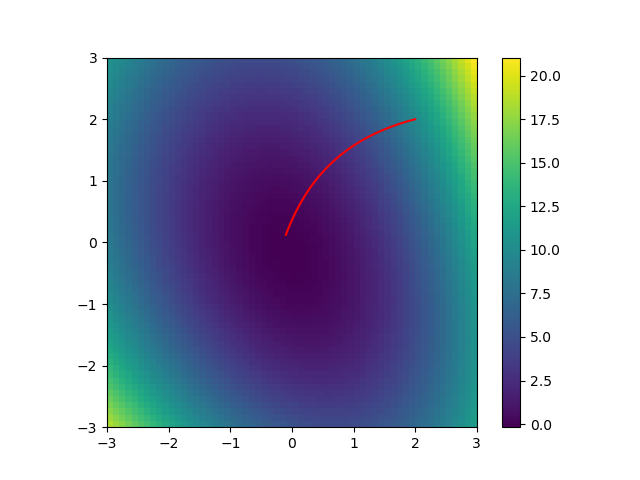
\includegraphics[width=0.8\linewidth]{imgs/optimize-fwd.png}
\caption{Using loma to optimize a 2D function.}
\label{fig:optimize}
\end{figure}

\paragraph{Optimizing a polynomial function.} The file \lstinline{examples/optimize_poly_fwd.py} implements a gradient descent optimization routine for a third order multivariate polynomial, where the gradient is computed using automatic differentiation. Figure~\ref{fig:optimize} shows the loss function landscape and the optimization trajectory (the red curve): we start from the top right (2, 2) and slowly move towards the center where the loss is lower.

\paragraph{Single pendulum derived using Hamiltonian mechanics.} 
We're going to use automatic differentiation to derive the equation of motion of a physical system, using something called Hamiltonian mechanics. This part is inspired by Justin Le's \href{https://github.com/mstksg/hamilton}{github project} and \href{https://blog.jle.im/entry/hamiltonian-dynamics-in-haskell.html}{blog post}.

Here, we are interested in a single pendulum, where the 2D location $(x, y)$ of the pendulum is dependent of a single angle $q$:
\begin{equation}
\begin{aligned}
x &= r \sin(q) \\
y &= -r \cos(q)
\end{aligned}
\end{equation}

Hamiltonian mechanics allows us to derive the equation of motion of the angle $q$, by adding an auxiliary variable $p$ (usually called the ``generalized momentum''), and positing two first-order ordinary differential equations over a \emph{Hamiltonian} $H(q, p)$:
\begin{equation}
\begin{aligned}
\dot{q} &= \frac{\partial}{\partial p} H(q, p) \\
\dot{p} &= -\frac{\partial}{\partial q} H(q, p)
\end{aligned}
\end{equation}

Our goal is to use automatic differentiation to automatically compute the two partial derivatives. First we need to define the Hamiltonian $H$.

The Hamiltonian $H$ is composed of two parts: the kinetic energy $K$ and the potential energy $U$.
\begin{equation}
H = K + U
\end{equation}

We set the potential energy to the gravitional potential energy:
\begin{equation}
U = m g y = -m g r \cos(q)
\end{equation}

The kinetic energy $K$ is a bit more involved, since we need to write it in terms of the generalized momentum $p$. See \href{https://blog.jle.im/entry/hamiltonian-dynamics-in-haskell.html}{Justin Le's blog post} for the derivation:
\begin{equation}
K = \frac{1}{2}m \left(\dot{x}^2 + \dot{y}^2\right) = \frac{1}{2} \mathbf{p}^T \left(J^T M J\right)^{-1} \mathbf{p}
\end{equation}
where
\begin{equation}
J=
\begin{bmatrix}
\frac{\partial x}{\partial q} \\
\frac{\partial y}{\partial q}
\end{bmatrix},
\end{equation}
,
\begin{equation}
M=
\begin{bmatrix}
m & 0 \\
0 & m
\end{bmatrix},
\end{equation}
and $\mathbf{p}$ is a length-1 vector that contains a single element $p$.

Even though the equations are involved, you can see that the $K$ function can be completely determined by everything above, so it's possible to completely automate the computation of $K$, while using automatic differentiation to compute $J$. Unfortunately, our system does not support nested differentiation yet (we need to differentiate $K$ later to compute the partial derivative of $H$), so here we'll compute it by hand: the (1-by-1) matrix $J^TMJ$ is:
\begin{equation}
J^TMJ = 
\begin{bmatrix}
m r^2
\end{bmatrix}
\end{equation}
So it's inverse is $\frac{1}{mr^2}$:
\begin{equation}
K = \frac{p^2}{mr^2}
\end{equation}

We can then implement the Hamiltonian in loma:
\begin{lstlisting}[language=Python]
class PendulumConfig:
    mass : float
    radius : float
    g : float

def hamiltonian(q : In[float], p : In[float], c : In[PendulumConfig]) -> float:
    K : float = p * p / (c.mass * c.radius * c.radius)
    y : float = -c.radius * cos(q)
    U : float = c.mass * c.g * y
    return K + U

d_hamiltonian = fwd_diff(hamiltonian)

def dHdq(q : In[float], p : In[float], c : In[PendulumConfig]):
    d_q : Diff[float]
    d_q.val = q
    d_q.dval = 1.0
    d_p : Diff[float]
    d_p.val = p
    d_p.dval = 0.0
    # dvals are automatically initialized to zero
    d_c : Diff[PendulumConfig]
    d_c.mass.val = c.mass
    d_c.radius.val = c.radius
    d_c.g.val = c.g
    return d_hamiltonian(q, p, c).dval

# dHdp is omitted
\end{lstlisting}

See \lstinline{examples/single_pendulum_fwd.mp4} for the animation in action.

\end{document}
